\documentclass{article}
\usepackage{ucs} 
\usepackage[utf8x]{inputenc} 	
\usepackage[czech]{babel}
\usepackage{pdfpages}
\usepackage{graphicx}
\usepackage{datetime}
\usepackage{titlesec}
\newcommand*\wildcard[2][5cm]{\vspace*{2cm}\parbox{#1}{\hrulefill\par#2}}  

\title{TuxMan - FPGA}
\titleformat{\paragraph}
\date{11/4/2019}
\author{Martin Přívozník}

\begin{document}
  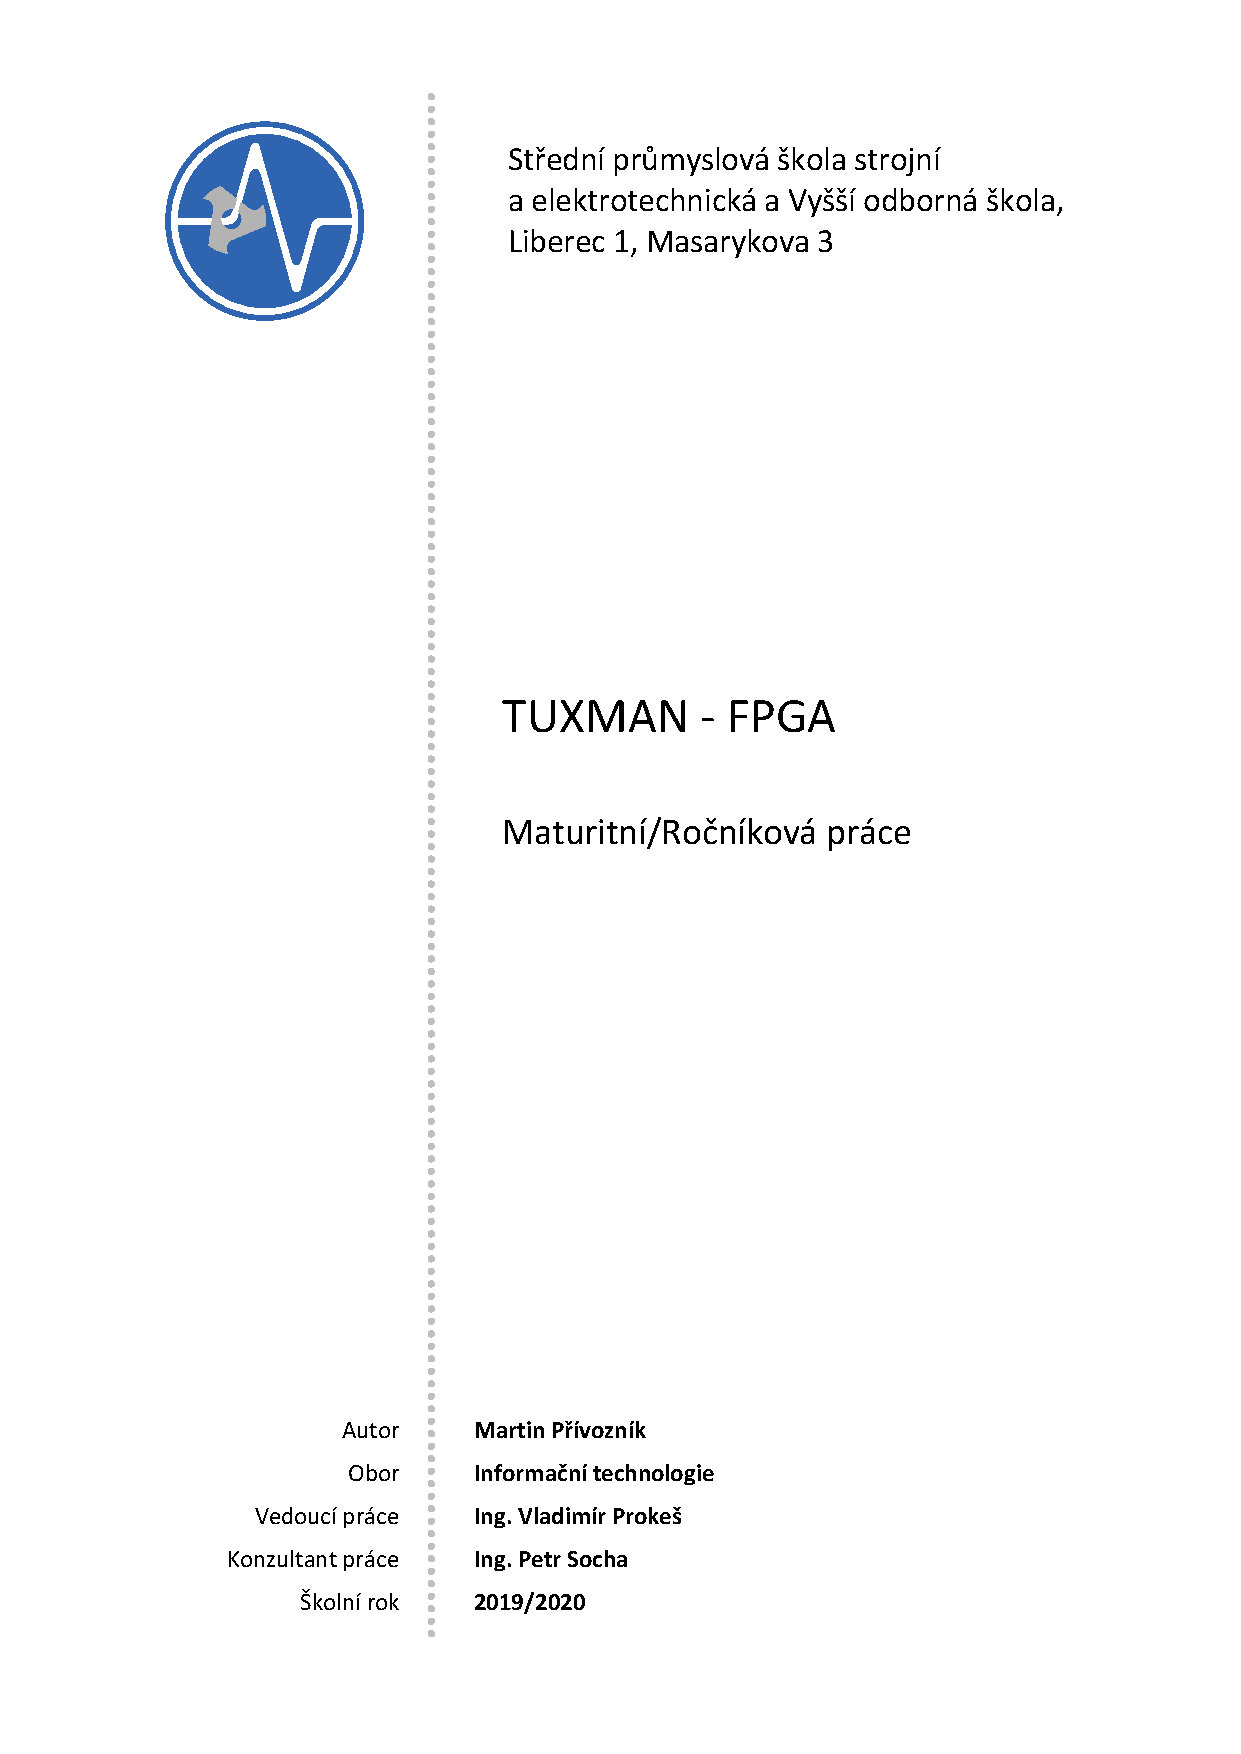
\includepdf[page={1}]{Front-Page}
  \newpage
  \pagenumbering{gobble}

 \section*{Anotace (Resumé)}
 Tématem práce je návrh arkádové hry na RTL úrovni a její implementace na programovatelném hradlovém poli, tj. FPGA. Uživatelský vstup je zajištěn pomocí PS/2 klávesnice a výstup prostřednictvím VGA. K implementaci je použit jazyk VHDL.

\section*{Klíčová slova}
RTL, programovatelné hradlové pole, FPGA, PS/2, VGA, VHDL

 \section*{Summary}
 The topic of this thesis is designing an arcade game on an RTL level and its implementation on a programmable gate array, i.e. FPGA. User input is provided by PS/2 keyboard and output is shown using VGA. Language called VHDL is used for implementation.

\section*{Keywords}
RTL, programmable gate array, FPGA, PS/2, VGA, VHDL

 \newpage
\vspace*{\fill}

 \section*{Čestné prohlášení}
 Prohlašuji, že jsem předkládanou maturitní/ročníkovou práci vypracoval sám a uvedl jsem veškerou použitou literaturu a bibliografické citace.

\vspace{ 2cm}
  V Liberci dne \today
  \hspace{2cm}
  \wildcard{Martin Přívozník}

\newpage
\tableofcontents

\newpage
\pagenumbering{arabic}

 \section*{Úvod}
 \addcontentsline{toc}{section}{Úvod}
 Něco pěknýho k úvodu, asi proč to dělám a tak ..

\section{Analýza}
Problematika FPGA ...
\subsection{VGA}
VGA is ...
\subsection{PS/2}
PS/2 is ...
\section{Neco}

\end{document}